\documentclass[a4paper,twoside,twocolumn]{article}

\usepackage[small]{cwpuzzle}
\usepackage{supertabular}         % Crossword clues to split over pages
\usepackage{rotating}             % For the inverted crossword answers
\usepackage{booktabs}             % For tables with TOPRULE, MIDRULE and BOTTOMRULE
\usepackage{graphicx}             % For various illustrations
\usepackage{wrapfig}
\usepackage{eurosym}
\usepackage{hyperref}             % For hyperlinks
\usepackage{verbatim}             % For the comment environment

\usepackage{url} % Used in JW's bin files

% Packages for article on Greek
\usepackage{amssymb}
\usepackage{textcomp}
\usepackage{bm}  % Bold math package for bold lowercase Greek
\usepackage[greek,english]{babel}
% \usepackage{fixmath}

% #----------------------------------------------------------------------------------
% Baskerville Definitions

\def \ukt {UK-TUG}

\newcommand{\BV}{\textit{Baskerville}}
\newcommand{\ISSUE}{10.2}
\newcommand{\ISSUEDATE}{October 2009}

% Used for author name at top of article
\newcommand{\AUTHOR}[1]
{
\textsf{#1} \vspace{1em}
}

\hyphenation{Bas-ker-ville}

% -----------------------------------------------------------------------------------
\font\manual=manfnt
\newcommand{\MF}{{\manual META}\-{\manual FONT}}
\newcommand{\MP}{\texttt{META}\-\texttt{POST}}

\newcommand{\BS}{$\backslash$}

% -----------------------------------------------------------------------------------
% Heading for pages after the first page.
\usepackage{fancyhdr}
\pagestyle{fancy}

% One heading per page, to the margin
\fancyhead[LO]{}
\fancyhead[LE]{\BV}                          
\fancyhead[RO]{\textit{Volume 10, Number 2}}
\fancyhead[RE]{}
\cfoot{-\thepage-}

\usepackage{bibunits}
%\usepackage{notes2bib}

% -----------------------------------------------------------------------------------
% Defintions and packages for "SIunitX" article.
%\usepackage{natbib}
\usepackage{siunitx} %,url}
\providecommand*\CTAN{\textsc{CTAN}}
\providecommand*\cs[1]{\texttt{\char`\\#1}}
\providecommand*\pkg[1]{\textsf{#1}}
\providecommand*\opt[1]{\texttt{#1}}

% -----------------------------------------------------------------------------------
% Defintions and packages for "ChemTex" article.
\usepackage{chemstyle,notes2bib,mciteplus} %} %rsc,siunitx,ur}
\usepackage[version=3]{mhchem}
\providecommand*\acro[1]{\textsc{#1}}
\providecommand*\BibTeX{\acro{Bib}\kern-.08em\relax\TeX}
\providecommand*\file[1]{\texttt{#1}}

% ============================================================================================
\begin{document}

\defaultbibliographystyle{plain}

% -----------------------------------------------------------------------------------
% PDF properties
% (Better here than in usepacakge because the latter loses spaces between words.)
\hypersetup{
  pdfauthor  = {Edited by Jonathan Webley},
  pdftitle   = {Baskerville \ISSUE},
  pdfsubject = {The Annals of the UK-TeX Users' Group}
}

% -----------------------------------------------------------------------------------
% Define a title page.
\begin{titlepage}
\begin{center}

\vspace{2cm}


\includegraphics[width=0.95\textwidth]{lion.png} \\ [2cm]

\textsc{\Large The Annals of the UK-\TeX\ Users' Group} \\[0.2cm]
{\large \href{http://uk.tug.org/}{uk.tug.org}} \\[0.2cm]
{\large ISSN 1354-5930}

\vfill

% Bottom of the page
{\large
\begin{tabular*}{0.9\textwidth}{@{\extracolsep{\fill}} l c r }
            & Edited by                 &             \\
Vol. \ISSUE & Jonathan \textsc{Webley}  & \ISSUEDATE  \\
\end{tabular*}}

\end{center}

\end{titlepage}

% -----------------------------------------------------------------------------------
\setcounter{tocdepth}{2}  % 2 = sub-sections
\tableofcontents

% ----------------------------------------------------------------------------------------
\vspace{0.5cm}
\noindent \textbf{\ukt\ Committee 2009}

\begin{itemize}
   \setlength{\parskip}{1pt} % Scrunch up to fit on first column
   \item Jonathan Fine (Chair)
   \item David Crossland (Secretary)
   \item David Saunders (Treasurer)
   \item Joseph Wright (Membership Secretary and Webmaster)
   \item John Trapp (Training Officer)
   \item Jonathan Underwood
   \item Charles Goldie
   \item Simon Dales
   \item Jonathan Webley (Baskerville Editor)
\end{itemize}
The  committee can be contacted at:
\begin{center}
\href{mailto:uktug-committee@uk.tug.org}{uktug-committee@uk.tug.org}
\end{center}

% ----------------------------------------------------------------------------------------
\section{Editorial}
Welcome to my second edition of \BV. I have been working on this edition, on and off, for months with various interruptions. It's been hard work and I've learnt a lot, but, finally, I've managed to pull everything together, and now we're up to twelve pages. I'm mentally planning the next edition for early next year, though that does depend on my availability and the quality and quantity of contributions.

%Unfortunately I will miss the AGM but wish it good luck nonetheless.

\hfill Jonathan Webley

\hfill \ \href{mailto:baskerville@uk.tug.org}{baskerville@uk.tug.org}

% ----------------------------------------------------------------------------------------
\section{Events}

% ----------------------------------------------------------------------------------------
\subsection{TUG 2010}

% 0.12 / 0.85

\begin{wrapfigure}{R}{0.2\textwidth}
    \vspace{-20pt} % Remove space at top of logo
    % [width=1.0\textwidth]
    
\includegraphics{tug_bw.jpg}
    \vspace{-10pt} % Remove space at boTtom of logo
\end{wrapfigure}


% Lots more material available on 2 emails or from website

TUG 2010 will be held in San Francisco, California, USA, from
  June 28--30, 2010, in the Sir Francis Drake Hotel in San Francisco.

Don Knuth and other members of the original Stanford \TeX\ Project will be there.  There will be several special events, including the conference banquet, to honour their work and celebrate \TeX's 32nd anniversary.

Abstracts and presentation proposals are welcome at any time, and hotel reservations are available. The registration form will be posted soon.

The official website is:
\begin{center}
 \href{http://tug.org/tug2010/}{tug.org/tug2010}
\end{center}


% ----------------------------------------------------------------------------------------
\section{News}
\subsection{The \TeX\ FAQ}
\emph{The UK List of \TeX\ Frequently Asked Questions on the Web} was updated in June this year and now contains 438 questions (and answers). The FAQ is maintained by Robin Fairbairns and is for English-speaking users of \TeX. The questions cover a wide range of topics, but the actual typesetting issues are mostly covered from the viewpoint of a \LaTeX\ user. 

The FAQ can be found at:
\begin{center}
\href{http://www.tex.ac.uk/faq}{www.tex.ac.uk/faq}
\end{center}

Any errors, corrections and potential new topics should be sent to:
\begin{center}
\href{mailto:faq-devel@tex.ac.uk}{faq-devel@tex.ac.uk}
\end{center}


% ----------------------------------------------------------------------------------------
\subsection{MathTran}

MathTran is a website that can be used to create, store and translate mathematical content. It translates mathematics entered using \TeX\ notation into images for inclusion in web pages and on emails. The latest version now allows users with an account to save their formulas.

MathTran is funded by the OU and JISC. The website can be found at:
\begin{center}
\href{http://www.mathtran.org/}{www.mathtran.org}
\end{center}


% ----------------------------------------------------------------------------------------
% \newpage
\section{The Hound}

\AUTHOR{Jonathan Webley}

% \vspace{3ex}

\begin{Puzzle}{11}{11}
|[1]C |E |R |I |[2]S |E |* |[3]A |[4]S |K |[5]S |.
|A |* |* |* |O |* |* |* |N |* |U |.
|[6]S |A |[7]C |* |[8]A |S |[9]S |U |A |G |E |.
|K |* |E |* |P |* |U |* |K |* |D |.
|[10]S |H |A |K |O |* |[11]P |I |E |C |E |.
|* |* |S |* |[12]P |I |E |* |P |* |* |.
|[13]S |T |E |L |E |* |[14]R |A |I |N |[15]Y |.
|H |* |F |* |R |* |H |* |T |* |O |.
|[16]A |N |I |M |A |T |E |* |[17]S |O |U |.
|G |* |R |* |* |* |R |* |* |* |T |.
|[18]S |M |E |W |* |[19]P |O |T |A |S |H |.
\end{Puzzle}

\noindent \textbf{Across} \\[2ex]
{\renewcommand{\arraystretch}{1.2}
\begin{tabular}{r p{6.7cm}}
 \textbf{1} & Inside the saucer, I see, is cherry-coloured. (6) \\
 \textbf{3} & Requests are listed in the task sheet. (4) \\
 \textbf{6} & I bought a bag in the Trossachs. (3) \\
 \textbf{8} & Sadly, use a gas mask to relieve pain. (7) \\
 \textbf{10} & Large hat, squashed, has okay from me. (5) \\
 \textbf{11} & Species, drowning without a ship, have no part. (5) \\
 \textbf{12} & This type of chart sounds like 3.14159 \dots (3) \\
 \textbf{13} & There's an obelisk of steel, rusted. (5) \\
 \textbf{14} & Lost in Iran, unknown at the end, wet. (5) \\
 \textbf{16} & Quicken the best, but meant badly. (7) \\
 \textbf{17} & So you want a coin? (3) \\
 \textbf{18} & Duck mews annoyingly. (4) \\
 \textbf{19} & Ah, the post was mislaid because it contains potassium. (6) \\
\end{tabular}}

\noindent \textbf{Down} \\[2ex]
{
\renewcommand{\arraystretch}{1.2}
\begin{tabular}{r p{6.7cm}}
 \textbf{1} & Kegs for 100 demands. (5) \\
 \textbf{2} & Sapper, with a double-O rating, watches a show. (4,5) \\
 \textbf{4} & A skin pest disfigures in dangerous places. (5,4) \\
 \textbf{5} & European sounds like leather. (5) \\
 %\end{tabular}
 %\begin{tabular}{r p{6.7cm}}
 \textbf{7} & You! Extinguish the flames and stop fighting. (9) \\
 \textbf{9} & Robin is found washed up on pure shore. (9) \\
 \textbf{13} & Cormorants burp gas. Sh! (5) \\
 \textbf{15} & Why art thou so young? (5) \\
\end{tabular}}

% ----------------------------------------------------------------------------------------

\section{\pkg{siunitx}: A \LaTeX\ Swiss army knife for units}
\begin{bibunit}
\AUTHOR{Joseph Wright}

%\begin{abstract}
\subsection{Introduction}
The \pkg{siunitx} package is a complete system for typesetting
units in \LaTeX.  It provides a large number of settings,
allowing the user complete control of the output for a fixed
input.  The package grew out of \pkg{SIunits} and
\pkg{SIstyle}, but covers many additional areas.  This article
provides a brief overview of why the new package was written
and some of its key features.
%\end{abstract}

\subsection{Background}

In November 2007, a seemingly simple query about a bug in the
\pkg{SIunits} package \cite{Heldorn2007} was posted to
\texttt{comp.text.tex}. I suggested a bug fix, but on
contacting the author of \pkg{SIunits} found he had no time for
further maintenance.  I therefore found myself somewhat
accidentally as the new package maintainer.  After fixing the
bug at hand, I decided to have a good look over the code, and
to ask for suggestions for improvements.  It soon became very
clear that unit support in \LaTeX\ needed serious attention,
and that tweaks to \pkg{SIunits} would not be enough.  At that
point, \pkg{siunitx} was born.

\subsection{Units in print}

The need for packages to control printing units is not
immediately obvious.  However, the existence of \pkg{SIunits},
\pkg{SIstyle} \cite{Els2006}, \pkg{fancyunits}
\cite{Bauke2007}, \pkg{unitsdef} \cite{Happel2005} and
\pkg{units} \cite{Reichert1998} attests to the desire to go
beyond direct input of units (and values).

Units are important, and without clear rules problems almost
automatically arise.  There are therefore internationally
agreed units: the \emph{Syst\`eme International d'Unit\'es}
\cite{BIPM2008}, usually referred to as SI units.  To go with
the agreed units are a set of rules on how to print both units
and the associated values; the National Institute of Standards and Technology (\textsc{nist}) have a good set of
guidelines for authors \cite{NIST2008}.  Doing this properly
and consistently is much better achieved using pre-build
macros, rather than checking every single use by hand.

At the same time, different publishers have their own conventions.
These do not always follow the `official' rules, and authors
do not want to change their source for every different use.
This again makes the strong case for using adjustable macros
for writing units; changing the style is then only a question
of altering the definition.

Finally, values as well as units have rules, and these rules
vary depending on publisher and country.  The \pkg{numprint}
package \cite{Harders2008} provides a range of tools to
automatically format numbers, to match the desired output
style.  It also includes basic abilities to include units with
these numbers.

\subsection{Enter \pkg{siunitx}}

Given the existing range of packages, the question arises `why
another package?'  The answer is that, although there are
several other packages, none covers everything. For example,
\pkg{SIunits} provides macros such as \cs{metre} to maintain
consistency, but is poor on control of numbers, whereas
\pkg{SIstyle} is stronger on numbers but does not provide unit
macros.  So a combined package, which can do everything, seemed
desirable.  Many of the ideas that I and others had were also
well beyond anything available in the existing solutions.  That
said, a lot of the internals of \pkg{siunitx} is taken
more-or-less verbatim from the existing packages.  The
\pkg{numprint} system has been extensively recycled here; most
of the number-interpreting system is based on the
\pkg{numprint} method.  Indeed, while the initial aim of the
new package was to deal primarily with \emph{units}, much of
the work I have undertaken has been concerned with
\emph{numbers}.

The design of \pkg{siunitx} is intended to be flexible.  Almost
everything is made available as an option, and given the number
of options, key--value controls were the only way to do this.
The package documentation covers (hopefully) all of them, but a
few examples here will illustrate the ideas.

\subsubsection{Some basics}

The basic macro of the package is \cs{SI}.  This takes a unit
and a value, and typesets them together.  The font used for
this is controlled, and the space between them cannot be
broken.  Thus for example \verb|\SI{10}{\metre}| gives
`\SI{10}{\metre}'.  The second argument is a unit, which can
be given as a series of macros, or can be literal text:
\verb|\SI{2}{N.m^2}| gives `\SI{2}{N.m^2}'.  Here, there is
no need to instruct the package to use maths mode for
superscripts: this is handled automatically.

Both the number and unit parts of the input can be used
independently, with macros \cs{num} and \cs{si}, respectively.
The \cs{num} macro can interpret and format a wide range of
numerical input.  So \verb|\num{1e2,3}| gives `\num{1e2,3}'
(when using U.K.~settings, at least).  As with the rest of the
package, the way that numbers are interpreted can be adjusted
by setting the appropriate package options.  For angles, the
\cs{ang} macro is available; it can work with angles as decimal
and arcs: \verb|\ang{1.23}| and  \verb|\ang{1;2;3}| give
`\ang{1.23}' and `\ang{1;2;3}', respectively.

Package options can be set in three ways.  As with most
packages, load-time options are recognised.  There is also a
\cs{sisetup} macro, which adjusts settings for all subsequent
input.  Finally, all of the user macros accept an optional
first argument; this allows changes for a specific item only.

\subsubsection{The unit processor}

One of the new ideas in \pkg{siunitx} is the unit processor.
This takes macro-based units, and can reformat them depending
on the desired output.  `Out of the box',
\verb|\SI{30}{\metre\per\second}| gives
`\SI{30}{\metre\per\second}', whereas if we set the option
\opt{per=slash}, the same input gives
`\SI[per=slash]{30}{\metre\per\second}'. This can be extended
further, allowing the interpretation of powers, including
reciprocals.  Thus, given the input
\verb|\SI{20}{\per\Square\second}|, the result can be
`\SI{20}{\per\Square\second}',
`\SI[per=slash]{20}{\per\Square\second}',
`\SI[per=frac]{20}{\per\Square\second}' or
`\SI[per=frac,fraction=nice]{20}{\per\Square\second}',
depending on the options set.

\subsubsection{Special effects}

A lot of work has gone into making more complex ideas available
for users of \pkg{siunitx}.  Thus the idea of `repeated'
units is easily handled:
\begin{verbatim}
\SI{1 x 2 x 3}{\metre}
\end{verbatim}
yields `\SI{1x2x3}{\metre}', for example.  Setting option
\opt{repeatunits=false}, the alternative (and not entirely
desirable) `\SI[repeatunits=false]{1x2x3}{\metre}' results.

Similarly, the conversion of angles between decimal and
degree--minute--second format is possible.  So
\verb|\ang{1.23}| normally gives the expected `\ang{1.23}';
setting \opt{angformat=arc} gives the alternative form
`\ang[angformat=arc]{1.23}'.

In many parts of the natural sciences, errors in physical
measurements are important.  Two ways are common for showing
these, as a separate error part, and as a bracketed error in
the last digit: \num[seperr]{1.23(4)} and \num{1.24(4)},
respectively.  Using \pkg{siunitx}, both forms can result from
the same input: \verb|\num{1.24(4)}|.  The separated form is
obtained by setting the \opt{seperr} flag.  This works with
exponents and units, for example:
\begin{verbatim}
\SI[seperr]{1.23(4)e5}{\candela}
\end{verbatim}
gives `\SI[seperr]{1.23(4)e5}{\candela}'.  Notice the
automatic addition of brackets to prevent ambiguity: this is an
adjustable package option.

The final extra to highlight is the provision of a new column
for tabular environments, the \texttt{S} column.  This brings
the ability to use the \cs{num} macro to tables, but also
brings control of alignment (including exponents).  A short
example shows the effect:
\begin{verbatim}
\begin{table}
  \centering
  \begin{tabular}{cS[tabformat=3.1]}
    \toprule
    {Entry} & {Distance/\si{\metre}} \\
    \midrule
    1 & 102.3 \\
    2 & 123.2 \\
    3 &   2,3 \\
    4 & 145.  \\
    5 &   2.3 \\
    \bottomrule
  \end{tabular}
\end{table}
\end{verbatim}
\begin{table}
  \centering
  \begin{tabular}{cS[tabformat=3.1]}
    \toprule
    {Entry} & {Distance/\si{\metre}} \\
    \midrule
    1 & 102.3 \\
    2 & 123.2 \\
    3 &   2,3 \\
    4 & 145.  \\
    5 &   2.3 \\
    \bottomrule
  \end{tabular}
\end{table}
Here, the contents of the \texttt{S} column are centred under
the column heading.  Space is reserved for three digits before
the decimal point, and one digit after.  Thus, while the
decimal points are aligned they are \emph{not} at the centre of
the column.  A range of options are provided to allow control
of positioning in \texttt{S} columns.

\subsubsection{Emulation}

Replacing the existing packages raises the issue of users
moving existing manuscripts to \pkg{siunitx}.  To aid this
transition, emulation modes are available for all of the
existing solutions.  This means that users of the existing
packages can experiment with \pkg{siunitx} without needing to
learn new default settings or input conventions.

\subsection{Conclusions}

This short article can only provide a flavour of the abilities
of \pkg{siunitx}.  However, it hopefully highlights the
possibilities made available by the new package.  The package
documentation includes a full range of examples, with almost
all of the package options illustrated.  I hope that I have
covered a wide range of needs, and that \pkg{siunitx} will make
it easier for \LaTeX\ users to get units right without working
too hard.  Suggestions for new features are always welcome,
particularly when they come with some interface ideas as well!

\putbib[siunitx]
\end{bibunit}

%\bibliography{siunitx}
%\bibliographystyle{unsrtnat}

\section{\LaTeX\ for chemists: filling in the gaps}
\begin{bibunit}
\AUTHOR{Joseph Wright} \\
%\begin{abstract}
\LaTeX\ is traditionally strongly favoured by mathematicians
and physicists.  Use by chemists has tended to remain on the
`physical' side of the subject.  Support for the particular
needs of chemists has therefore be somewhat variable.  I have
been involved with a selection of new or improved packages,
which seek to address some of the gaps.
%\end{abstract}

\subsection{Introduction}

\LaTeX\ has a whole range of packages available, aimed at
almost the entire range of (academic) pursuits.  However, gaps
still arise, and are filled by interested users.  For chemists,
despite the existence of some very useful tools, gaps have
remained.  As I have worked with \LaTeX, I have worked to fill
some of those gaps, as far as I have been able.  This article
gives an overview of the areas I have contributed to, as well
as highlights from others, and showing some gaps that remain.
All of my packages are available from \CTAN\ in the usual
manner: to keep the bibliography a little shorter, these are
not formally cited although other people's packages are.

Some chemistry-focussed packages will be mentioned in the rest
of this article.  However, one which deserves particular
mention here is \pkg{mhchem} \cite{Hensel2007}.  This allows
very simple input of chemical formulae (and simple in-line
equations). Thus, it allows you to write \verb|\ce{H2SO4}| to
get \ce{H2SO4}, \verb|\ce{CH2=CH-C#CH}| to get
\ce{CH2=CH-C#CH}, or
\begin{verbatim}
\ce{2H2 + O2 -> 2H2O}
\end{verbatim}
and get
\begin{equation}
  \ce{2H2 + O2 -> 2H2O}.
\end{equation} 
It is a tool no chemist using \LaTeX\ should be without.

\subsection{Bibliography tools}

\subsubsection{\BibTeX\ styles}

One area where chemists seem to have unusual requirements is in
creating bibliographies.  To begin with, as a chemist the name
is wrong: it is the \emph{References} section.  The most basic
requirement for everyone using \BibTeX\ is appropriate style
files.  When I started using \LaTeX, I found the
\file{pccp.bst} \BibTeX\ style, based on the journal
\emph{Physical Chemistry Chemical Physics}.  However, there
were problems with the output.  I therefore wrote my own style,
\file{rsc.bst}, based on the general requirements of the Royal
Society of Chemistry (\acro{RSC}); as a U.K.-based worker, the
\acro{RSC} style is one I follow for my own documents.  Over
time, \file{rsc.bst} was joined by \file{angew.bst}, aiming at
the requirements of \emph{Angewandte Chemie} (arguably the
`top' general chemistry journal: I'm sure a lot of American
chemists would disagree!). These files, plus some utility
macros, ended up in a package called \pkg{rsc}. Later, the
utility macros moved elsewhere, but the \pkg{rsc} survives in
modified form.

The \pkg{achemso} package was originally written by Mats
Dahlgren, and provided a \BibTeX\ style following the
requirements of the American Chemical Society (\acro{ACS}).
Once I started using the style, I spotted some issues.
Contacting the author, I found he no longer had time for
package maintenance.  So, as much by accident as by design, I
took over \pkg{achemso}.  A complete re-write resulted, with
improvement to the \BibTeX\ style and the accompanying \LaTeX\
package. More recently, I've re-written the package again so that
it fits in with the submission system at the \acro{ACS}: this
hopefully makes submitting articles a bit easier. 

\subsubsection{Bibliography packages}

Beyond \BibTeX\ styles, chemists have two important
requirements for bibliographies.  First, the idea of
`compound' references is common.  Most chemistry journals use
numerical citations, rather than the author--date system.
It is very common to want a single reference number to refer to
several related journal articles.  The \pkg{mcite} package
\cite{Ohl2005} can do this, but with very limited control of
the results. In particular, it's common in chemistry to give
each reference a letter inside a long list, such as
\begin{quote}
  [4] (\emph{a}) G.~Alberti, M.~Casciola, U.~Costantino,
  A.~Peraio and E.~Montoneri, \emph{Solid State Ionics}, 1992,
  \textbf{50}, 315--322; (\emph{b}) G.~Alberti, M.~Casciola,
  U.~Costantino and R.~Vivani, \ldots
\end{quote}
The \pkg{mcite} package cannot do this automatically.  So I
began to consider the issue, and to ask on
\texttt{comp.text.tex} if anyone had contact details for the
author of \pkg{mcite}. Luckily, Michael Shell was interested in
the other extensions to \pkg{mcite}: the result was the
\pkg{mciteplus} package \cite{Shell2008}, which \emph{can}
generate the desired output with control of formatting.
Although I did not write any of \pkg{mciteplus}, the aim of
making sub-lists inside each reference is included there
specifically because I worked with him to get it working. Thus
the example citation above can be given in the source simply as
\begin{verbatim}
\cite{Alberti1992,*Alberti1996}
\end{verbatim}
which results in nicely-formatted output
as above.
%\cite{Alberti1992,Alberti1996}.
This document uses my
\file{rsc.bst} \BibTeX\ style, which sets up \pkg{mciteplus}
to follow the requirements of the \acro{RSC}; for example, this
instructs \pkg{mciteplus} to use a sub-list, and to make the
sub-labels italic.

The second thing that chemists like to do is mix notes and
references.  This can be done by creating a \BibTeX\ database
of notes for every document you write to contain the
information, but it is tedious.  A much better idea would be to
add the text directly into the body of the file, and have it
move automatically to the bibliography section.  To achieve
this, I wrote the \pkg{notes2bib} package.  The package works
by creating a database for the notes during the \LaTeX\ run,
and then ensuring it is added to the list of files to be
processed by \BibTeX. This means it is `neutral' with respect
to sorting of bibliographies and packages used, such as
\pkg{cite} \cite{Arseneau2009}, \pkg{natbib} \cite{Daly2009},
\pkg{biblatex} \cite{Lehman2009}, etc.  Using \pkg{notes2bib}
implies using numerical citations: the citations do not make
much sense with the author--year system!  Using the package
requires only inclusion of one or more \cs{bibnote}s in the
source, although it is possible to convert \cs{footnote} or
\cs{endnote} entries into \cs{bibnote} data automatically.  For
example, you could write
\begin{verbatim}
\bibnote{An example bibliographic note}
\end{verbatim}
and this would give \bibnote{An example bibliographic note}.

\subsection{Utilities}

The \pkg{mhchem} package is probably the most useful general
utility package for chemists.  However, this leaves a few gaps
that can happily be filled.  Initially, I provided a package
with the \pkg{rsc} bundle to do this.  However, later it became
clear there was a better approach.  The \pkg{chemstyle} package
inherited the utilities from \pkg{rsc}, along with new
functions.  For example, this gives the macros \verb|\tBu|,
\verb|\iPr|, \etc. to give alkyl radicals: \tBu, \iPr, \etc. It
also provides items such as the `standard state' symbol, to
allow you to produce $\Delta H^{\standardstate}$ easily.

The main aim of \pkg{chemstyle} is to help maintain
consistency.  By specifying the journal style to follow, the
package allows float captions, cross-referencing and so on to
follow the choices of the publication given.  This is a lot
easier than trying to remember the choices of every separate
journal. It also loads a number of useful packages for the
chemist, including my own \pkg{chemscheme}.

\subsection{Graphics: the `scheme'}

The concept of a `scheme' is one that non-chemists find
difficult to understand: they expect the name `equation' to
be used.  An equation to most synthetic chemists is a simple,
broadly non-graphical item, such as Equation~\ref{eqn}.
\begin{equation}
  \ce{2H2 + O2 -> 2H2O} \label{eqn}
\end{equation}
In contrast, a scheme is a more complex, graphically-rich item,
such as \ref{sch}. The example here is simple by the standards
of many schemes in the research literature.  Several packages
are available for generating the graphics directly in \LaTeX.
However, producing anything beyond the most simple scheme
becomes very difficult using text-based tools.  I, like almost
every synthetic chemist, use the commercial package
\textsc{ChemDraw}\bibnote{See
\url{http://www.cambridgesoft.com}} to produce my schemes.
\begin{scheme}
  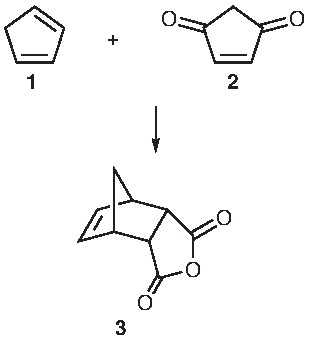
\includegraphics{Scheme}
  \caption{A simple scheme}
  \label{sch}
\end{scheme}

Rather than trying to provide a package to tackle directly
producing schemes in \LaTeX, the \pkg{chemscheme} package aims
to solve two lesser problems.  The first aim of
\pkg{chemscheme} is to provide an `out of the box' float for
schemes.  Chemists expect the scheme to be near `here' if
possible, so this is the case with the \texttt{scheme} float.
Thus the example scheme used here is produced using
\begin{verbatim}
\begin{scheme}
  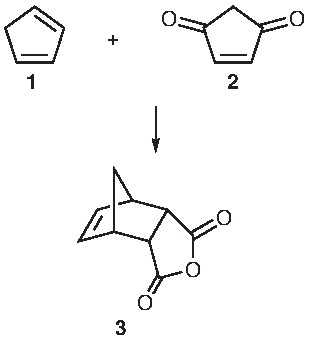
\includegraphics{Scheme}
  \caption{A simple scheme}
  \label{sch}
\end{scheme}
\end{verbatim}

The second aim is more complex.  The use of reference numbers
for chemicals in graphics is very common.  Two packages exist
to automate this in the text: \pkg{bpchem} \cite{Pedersen2004}
and \pkg{chemcompounds} \cite{Schenk2006}.  However, neither
can work with graphical content.  Using \pkg{PSfrag}
\cite{Carlisle1998}, the \pkg{chemscheme} package makes
automatic substitution easy for \file{.eps} graphics. This is
achieved by the \cs{schemeref} macro, which works with a
temporary marker in the input.  By using \pkg{pst-pdf}
\cite{Gasslein2008} this can also be used with PDF\LaTeX.

\subsection{\pkg{biblatex} bibliographies}

The \pkg{biblatex}, currently available with beta status, is a 
completely new way to produce bibliographies from a database. 
The current version uses \BibTeX, but does not need dedicated
style files to do this. Instead, it requires \LaTeX\ files containing
formatting instructions.  I've written some of these for chemists
and other scientists: \pkg{biblatex-chem} to cover the same journals
as \pkg{rsc} and \pkg{achemso}, \pkg{biblatex-nature} for 
\emph{Nature}-like formatting and \pkg{biblatex-science} to emulate
the journal \emph{Science}.

\subsection{Further afield}

Beyond the focus on chemistry, one package in particular
deserves mention here.  Using units with numbers is common
across the whole of science.  The \pkg{siunitx} package
provides a wide range of tools for typing units and values. For
example, the input
\begin{verbatim}
$R = \SI[dp=3]{8.314472}
  {\joule\per\mole\per\kelvin}$
\end{verbatim}
gives the typeset result $R = \SI [dp=3] {8.314472}
{\joule\per\mole\per\kelvin}$, while
\begin{verbatim}
$R = \SI[dp=5,per=slash]{8.314472}
  {\joule\per\mole\per\kelvin}$
\end{verbatim}
gives $R = \SI [dp=5,per=slash] {8.314472}
{\joule\per\mole\per\kelvin}$.  This type of format control is
available either on a per-macro basis or by setting package
settings in the document.  The aim of \pkg{siunitx} is
therefore to allow units and values to have a single input
syntax but give a range of output formats: this makes working
with different publishing requirements much easier.

\putbib[ChemTeX,niib-Baskerville10.2]
\end{bibunit}

% \bibliographystyle{rsc}
% \bibliography{ChemTeX}

\section{An Introduction to the Greek Alphabet}
\AUTHOR{Jonathan Webley} \\
The first pure alphabet emerged around 2000 BCE in Egypt, based on alphabetic principles of the Egyptian hieroglyphs and is called the Proto-Sinaitic alphabet. Surprisingly, nearly every alphabet in the world today either descends directly from it or was inspired by it.

Essentially, writing was independently invented only a handful of times. Virtually every symbol we see today in the West had as its ultimate origins the work of, probably, a single person, living in, probably, ancient Egypt. That idea was then copied and evolved and developed to become the tens of thousands of symbols, for example, found in Unicode.

An important descendant of the Proto-Sinaitic alphabet was the Phoenician alphabet, which in turn evolved into the Arabic, Hebrew and Greek alphabets. Indian scripts such as Devanagari are also descendants of the Phoenician alphabet. All the modern scripts of Europe -- such as Latin, Gothic and Cyrillic -- are descended from the Greek alphabet. Our word \emph{alphabet} derives from the Greek letters \emph{alpha} and \emph{beta}.

% -------------------------------
\subsection{Math mode}
Because of its widespread use in mathematics, science and engineering the Greek alphabet is a standard feature of \TeX\ when in math mode. There are codes for every lowercase letter except omicron, because it has the same shape as the Latin ``\texttt{o}''. The math mode versions of the lowercase Greek letters are in italics whereas the uppercase letters are upright.

\begin{figure}[h]
	\centering
		
\includegraphics[width=0.9\textwidth]
		            {Greek_Inscription.jpg}
	\caption*{Greek Inscription, 5th century BCE}
	\label{fig:Greek_Inscription}
\end{figure}



% -------------------------------
\subsection{Babel}
Using the \texttt{greek} option of the \texttt{Babel} package is the normal way to write text in Greek. If the whole document is in Greek then the preamble would include: \\
\indent $\backslash$\texttt{usepackage[greek]\{babel\}} \\
Each Latin letter in the \texttt{tex} file is then automatically transliterated to its equivalent Greek letter. These equivalences are given in the tables below.

A document such as this one, containing mainly English with a smattering of Greek, would have: \\
\indent $\backslash$\texttt{usepackage[greek,english]\{babel\}} \\
and in the body when Greek is required: \\
\indent $\backslash$\texttt{foreignlanguage\{greek\}\{Alpha\}} \\
which renders as \\
\indent \foreignlanguage{greek}{Alpha} \\
\LaTeX\ also has other ways of achieving the same result which are not detailed here.

The \texttt{greek} option of this package also includes three obsolete letters as illustrated below The \LaTeX\ codes for these letters are: $\backslash$\texttt{qoppa}, $\backslash$\texttt{sampi} and $\backslash$\texttt{stigma} and these are shown later.

% -------------------------------
\subsection{The Letters}
 There are 24 letters in the modern Greek alphabet, with uppercase and lowercase variants. These letters are given in the following tables, and the columns in it are:
\begin{enumerate}
	\item Greek letter produced in math mode by standard \TeX.
	\item The \TeX\ code for this letter (the letter name).
	\item Greek letter produced by the \texttt{Babel} package.
	\item The Latin letter used to produce this letter.
\end{enumerate}

\medskip
\begin{table}[H]
	\centering
	\caption* {Lowercase letters}
		\begin{tabular}{cp{3.2cm}cc}
		  \toprule
			\LaTeX\    & \LaTeX\   & Latin  & Latin \\
			letter          & code         & letter &       \\ 
\midrule
$\alpha$                  & \texttt{$\backslash$alpha}  & \foreignlanguage{greek}{a} & a \\
$\beta$                   & \texttt{$\backslash$beta}   & \foreignlanguage{greek}{b} & b \\
$\gamma$                  & \texttt{$\backslash$gamma}  & \foreignlanguage{greek}{g} & g \\
$\delta$                  & \texttt{$\backslash$delta}  & \foreignlanguage{greek}{d} & d \\
$\epsilon$, $\varepsilon$ & \texttt{$\backslash$epsilon},  \texttt{$\backslash$varepsilon} & \foreignlanguage{greek}{e} & e \\
$\zeta$                   & \texttt{$\backslash$zeta}   & \foreignlanguage{greek}{z} & z \\
$\eta$                    & \texttt{$\backslash$eta}    & \foreignlanguage{greek}{h} & h\\
$\theta$, $\vartheta$     & \texttt{$\backslash$theta}, \texttt{$\backslash$vartheta} & \foreignlanguage{greek}{j} & j \\
$\iota$                   & \texttt{$\backslash$iota}   & \foreignlanguage{greek}{i} & i \\
$\kappa$                  & \texttt{$\backslash$kappa}  & \foreignlanguage{greek}{k} & k \\
$\lambda$                 & \texttt{$\backslash$lambda} & \foreignlanguage{greek}{l} & l \\
$\mu$                     & \texttt{$\backslash$mu}     & \foreignlanguage{greek}{m} & m \\
$\nu$                     & \texttt{$\backslash$nu}     & \foreignlanguage{greek}{n} & n \\
$\xi$                     & \texttt{$\backslash$xi}     & \foreignlanguage{greek}{x} & x \\
$o$                       & o (omicron)                 & \foreignlanguage{greek}{o} & o \\
$\pi$, $\varpi$           & \texttt{$\backslash$pi}, \texttt{$\backslash$varpi}      &  \foreignlanguage{greek}{p} & p \\
\bottomrule
		\end{tabular}
\end{table}

\begin{table}[H]
	\centering
	\caption* {Lowercase letters (cont.)}
		\begin{tabular}{cp{3.2cm}cc}
		  \toprule
			\LaTeX\    & \LaTeX\   & Latin  & Latin \\
			letter          & code         & letter &       \\ 
\midrule
$\rho$, $\varrho$         & \texttt{$\backslash$rho}, \texttt{$\backslash$varrho}    & \foreignlanguage{greek}{r}  & r \\
$\sigma$, $\varsigma$     & \texttt{$\backslash$sigma}, \texttt{$\backslash$varsigma} & \foreignlanguage{greek}{s} & s \\
$\tau$                    & \texttt{$\backslash$tau}                                  & \foreignlanguage{greek}{t} & t \\
$\upsilon$                & \texttt{$\backslash$upsilon}                              & \foreignlanguage{greek}{u} & u \\
$\phi$, $\varphi$         & \texttt{$\backslash$phi}, \texttt{$\backslash$varphi}     & \foreignlanguage{greek}{f} & f \\
$\chi$                    & \texttt{$\backslash$chi}                                  & \foreignlanguage{greek}{q} & q \\
$\psi$                    & \texttt{$\backslash$psi}                                  & \foreignlanguage{greek}{y} & y \\
$\omega$                  & \texttt{$\backslash$omega}                                & \foreignlanguage{greek}{w} & w \\
\bottomrule
		\end{tabular}
\end{table}
\medskip

Many of the uppercase letters are simply those used in the Latin alphabet, and for these there is no \TeX\ code. In this case, the letter name is given in brackets.

\medskip
\begin{table}[H]
	\centering
	\caption* {Uppercase letters}
		\begin{tabular}{cp{2.5cm}cc}
		  \toprule
			\LaTeX\    & \LaTeX\   & Latin  & Latin \\
			letter          & code         & letter &       \\ 
\midrule
A            & A (alpha)                    & \foreignlanguage{greek}{A} & A \\
B            & B (beta)                     & \foreignlanguage{greek}{B} & B \\
$\Gamma$     & \texttt{$\backslash$Gamma}   & \foreignlanguage{greek}{G} & G \\
$\Delta$     & \texttt{$\backslash$Delta}   & \foreignlanguage{greek}{D} & D \\
E            & E (epsilon)                  & \foreignlanguage{greek}{E} & E \\
Z            & Z (zeta)                     & \foreignlanguage{greek}{Z} & Z \\
H            & H (eta)                      & \foreignlanguage{greek}{H} & H \\
$\Theta$     & \texttt{$\backslash$Theta}   & \foreignlanguage{greek}{J} & J \\
I            & I (iota)                     & \foreignlanguage{greek}{I} & I \\
K            & K (kappa)                    & \foreignlanguage{greek}{K} & K \\
$\Lambda$    & \texttt{$\backslash$Lambda}  & \foreignlanguage{greek}{L} & L \\
M            & M (mu)                       & \foreignlanguage{greek}{M} & M \\
N            & N (nu)                       & \foreignlanguage{greek}{N} & N \\
$\Xi$        & \texttt{$\backslash$Xi}      & \foreignlanguage{greek}{X} & X \\
O            & O (omicron)                  & \foreignlanguage{greek}{O} & O \\
$\Pi$        & \texttt{$\backslash$Pi}      & \foreignlanguage{greek}{P} & P \\
P            & P (rho)                      & \foreignlanguage{greek}{R} & R \\
$\Sigma$     & \texttt{$\backslash$Sigma}   & \foreignlanguage{greek}{S} & S \\
T            & T (tau)                      & \foreignlanguage{greek}{T} & T \\
$\Upsilon$   & \texttt{$\backslash$Upsilon} & \foreignlanguage{greek}{U} & U \\
$\Phi$       & \texttt{$\backslash$Phi}     & \foreignlanguage{greek}{F} & F \\
X            & X (chi)                      & \foreignlanguage{greek}{Q} & Q \\
$\Psi$       & \texttt{$\backslash$Psi}     & \foreignlanguage{greek}{Y} & Y \\
$\Omega$     & \texttt{$\backslash$Omega}   & \foreignlanguage{greek}{W} & W \\
\bottomrule
		\end{tabular}
\end{table}

\medskip

There is also a variant of kappa found in the \texttt{amssymb} package: $\varkappa$ (\texttt{\$$\backslash$varkappa}\$).

% -------------------------------
\subsection{Obsolete letters}
There are a number of obsolete letters. The samples in the following table derive either from \texttt{amssymb} or from the \texttt{greek} option of the \texttt{Babel} package.

The \texttt{arevmath} package is intended for presentations and posters and its use is not illustrated here. There are large and small forms of each letter, which otherwise seem identical.

\medskip
\begin{center}
\begin{tabular}{lcp{3.5cm}}
\toprule
Name & Letter & Packages \\
\midrule
digamma & $\digamma$                       & amssymb, arevmath  \\
het     &                                  & none known \\
koppa   &                                  & arevmath           \\
qoppa   & \foreignlanguage{greek}{\qoppa}  & arevmath, babel    \\
sampi   & \foreignlanguage{greek}{\sampi}  & arevmath, babel    \\
san     &                                  & none known \\
sho     &                                  & none known \\
stigma  & \foreignlanguage{greek}{\stigma} & arevmath, babel    \\
\bottomrule
\end{tabular}
\end{center}
\medskip

Qoppa and koppa refer to the same letter: its shape evolved from that referred to as qoppa to that referred to as koppa.

All of these letters are available in Unicode.

% -------------------------------
\subsection{Greek Diacritics}
Modern Greek uses only two diacritics, however, before 1982 Greek orthography was more complex. Modern Greek is called monotonic (meaning ``single accented''), while the older orthography is called polytonic (meaning ``many accented''). The Babel package by default uses the modern orthography, but the following preamble allows the older orthography to be used: \\
\indent $\backslash$\texttt{usepackage[greek]\{babel\}} \\
\indent $\backslash$\texttt{languageattribute\{greek\}\{polutoniko\}} \\
The latter option, ``polutoniko'', is the Greek for ``polytonic''.


Use of this option is not illustrated here.

% -------------------------------
\subsection{Some uses}
A couple of letters can be found in the \texttt{textcomp} and \texttt{gensymb} packages:

\medskip

\begin{center}
\begin{tabular}{ccc}
\toprule
Symbol   & textcomp & gensymb \\
\midrule
\textohm & $\backslash$textohm & $\backslash$ohm \\
\textmu  & $\backslash$textmu  & $\backslash$micro \\
\bottomrule
\end{tabular}
\end{center}

\medskip

This version of \textit{mu} is used for the SI prefix micro- for $10^{-6}$. For example, the symbol for a micron is \texttt{\textmu m}.

Mathematics uses variants of \textit{sigma} and \textit{pi} as operators, such that in display mode subscripts and superscripts are placed beneath or above the letters respectively. These symbols are found in the \texttt{amssymb} package:

\begin{tabular}{cc}
$\displaystyle \sum_{i=0}^{n}$  & \texttt{\$$\backslash$sum\_\{i=0\}\^{}n\$} \\
$\displaystyle \prod_{i=0}^{n}$ & \texttt{\$$\backslash$prod\_\{i=0\}\^{}n\$}
\end{tabular}

A couple of symbols are inverted, and are found in the \texttt{amssymb} package:

\begin{tabular}{clp{4.2cm}}
$\mho$   & \texttt{$\backslash$mho}   & This is ohm spelt backwards, and is an unofficial symbol for the siemens. \\
$\nabla$ & \texttt{$\backslash$nabla} & This symbol is the \textit{del} operator in mathematics.
\end{tabular}


\subsection{Greek Arithmetic}
In Greek, there are no separate symbols. glyphs, for numbers. Modern Greek uses the same arabic numerals that we use. So, like the Romans, the ancient Greeks used letters to stand for numbers (unlike the arabic system where the symbols stand for digits). 

The earliest system used was the Attic system, which is similar to the system used by the Romans:

\medskip

\begin{center}
\begin{tabular}{rcc}
\toprule
 Arabic & Greek & Roman \\
\midrule
 1     & I         & I \\
 5     & $\Pi$     & V \\
10     & $\Delta$  & X \\
100    & H         & C \\
1,000  & X         & M \\
10,000 & M         &   \\
\bottomrule
\end{tabular}
\end{center}

\medskip

The letters used by the Greeks are the initial letters of the words for the numbers. Each letter represents a number, and the values are added (though the Romans also subtracted):
\[
4 = \text{IIII (Greek)} = \text{IV (Roman)}
\]

A later system was the Ionian or Athenian system, which uses 27 letters (the modern 24 letters plus 3 obsolete letters):

\medskip

\begin{center}
\begin{tabular}{lrclrclr}
%\toprule
% Letter & Number \\
%\midrule
$\alpha$   & 1  && $\iota$    & 10 && $\rho$     & 100 \\
$\beta$    & 2  && $\kappa$   & 20 && $\sigma$   & 200 \\
$\gamma$   & 3  && $\lambda$  & 30 && $\tau$     & 300 \\
$\delta$   & 4  && $\mu$      & 40 && $\upsilon$ & 400 \\
$\epsilon$ & 5  && $\nu$      & 50 && $\phi$     & 500 \\
$\digamma$ & 6  && $\xi$      & 60 && $\chi$     & 600 \\
$\zeta$    & 7  && o          & 70 && $\psi$     & 700 \\
$\eta$     & 8  && $\pi$      & 80 && $\omega$   & 800 \\
$\theta$   & 9  && \foreignlanguage{greek}{\qoppa} & 90 && \foreignlanguage{greek}{\sampi} & 900 \\
%\bottomrule
\end{tabular}
\end{center}

This system is also additive. So, $123 = \rho\kappa\alpha$. Extensions to this system allow for larger numbers.

Package \texttt{$\backslash$athnum} can be used to convert numbers in arabic format to numbers in Ionian format.

\medskip


% ----------------------------------------------------------------------------------------
\section{The Hound Answers}

\noindent \textbf{Across} \\
\begin{turn}{180} 
 16. animate,
 17. sou,
 18. smew,
 19. potash
\end{turn} \\
\begin{turn}{180}
 10. shako,
 12. pie,
 13. stele,
 14. rainy,
 \end{turn} \\
\begin{turn}{180}
 1. cerise,
 3. asks,
 6. sac,
 8. assuage,
 11. piece,
\end{turn} \\

\noindent \textbf{Down} \\
\begin{turn}{180}
15. youth
\end{turn} \\
\begin{turn}{180}
5. suede,
7. ceasefire,
9. superhero,
13. shags,
\end{turn} \\
\begin{turn}{180}
1. casks,
2. soap opera,
4. snake pits,
\end{turn}

% -----------------------------------------------------------------------------------
\section{Contributions}
\noindent All contributions to \BV\ should be sent to the editor at:
\begin{center}
\href{mailto:baskerville@uk.tug.org}{baskerville@uk.tug.org}
\end{center}

Articles on any area of \TeX\ or its friends, \ukt\ or related topics are very welcome. The Committee is particularly keen to publish articles with a UK \textit{flavour}. Send in your comments on this issue; your suggestions, letters, thoughts, tips and hints, articles, jokes, questions, requests for help, jobs, cartoons or puzzles -- anything relevant will be considered for publication.

%The deadline for the next issue is [\textbf{DATE}]. 

\end{document}

